\documentclass[11pt]{article}
\usepackage[T1]{fontenc}
\usepackage{newtxtext}
\usepackage{amsmath,amssymb,mathtools,amsthm}
\usepackage{newtxmath}
\input{glyphtounicode}
\input{glyphtounicode-cmex}
\pdfglyphtounicode{barex}{007C}
\pdfglyphtounicode{parenlefttpA}{239B}
\pdfglyphtounicode{parenrighttpA}{239E}
\pdfglyphtounicode{parenleftbtA}{239D}
\pdfglyphtounicode{parenrightbtA}{23A0}
\pdfglyphtounicode{parenleftexA}{239C}
\pdfglyphtounicode{parenrightexA}{239F}
\pdfgentounicode=1
\usepackage[margin=1in]{geometry}
\usepackage{microtype}
\usepackage{booktabs,array}
\usepackage[dvipsnames]{xcolor}
\usepackage{graphicx,tikz}
\usepackage{enumitem,needspace}
\usepackage{textcomp,listings}
\usepackage[colorlinks=true,linkcolor=MidnightBlue,citecolor=MidnightBlue,urlcolor=MidnightBlue]{hyperref}
\hypersetup{pdftitle={Exact Fourier certificates for complex Hadamard matrices of order six},pdfauthor={OpenAI}}
\setlist{itemsep=2pt,topsep=5pt}
\newtheorem{theorem}{Theorem}[section]
\newtheorem{lemma}[theorem]{Lemma}
\newtheorem{proposition}[theorem]{Proposition}
\newtheorem{corollary}[theorem]{Corollary}
\theoremstyle{definition}
\newtheorem{definition}[theorem]{Definition}
\theoremstyle{remark}
\newtheorem{remark}[theorem]{Remark}
\newcommand{\C}{\mathbb C}
\newcommand{\T}{\mathbb T}
\newcommand{\Z}{\mathbb Z}
\newcommand{\Q}{\mathbb Q}
\newcommand{\E}{\mathbb E}
\DeclareMathOperator{\Ree}{Re}
\DeclareMathOperator{\ord}{ord}
\DeclareMathOperator{\tr}{Tr}
\DeclareMathOperator{\diag}{diag}
\setlength{\emergencystretch}{1em}
\lstdefinestyle{certificate}{
  language=Python,
  basicstyle=\fontsize{7.7}{9.1}\selectfont\ttfamily,
  keywordstyle=\bfseries,
  commentstyle=\color{black!65},
  stringstyle=\color{black},
  numbers=left,
  numberstyle=\fontsize{6.5}{8}\selectfont\color{black!60},
  numbersep=6pt,
  columns=fullflexible,
  keepspaces=true,
  showstringspaces=false,
  upquote=true,
  breaklines=true,
  breakatwhitespace=false,
  tabsize=4,
  xleftmargin=15pt,
  frame=none,
  aboveskip=10pt,
  belowskip=10pt
}


\title{Exact Fourier certificates for complex Hadamard matrices of order six}
\author{OpenAI}
\date{September 24, 2026}

\begin{document}
\maketitle

\begin{abstract}
We prove the Fourier-vanishing conjecture of Matolcsi, Ruzsa, and Weiner:
every complex Hadamard matrix of order six outside Tao's cubic equivalence
class has a vanishing character sum at every permutation of
$(1,1,1,-1,-1,-1)$. We also give an exact certificate excluding seven
mutually unbiased bases in $\C^6$; by Weiner's completion theorem, this
yields an upper bound of five. Both certificates use only integer and
rational arithmetic, and the complete verifier is included.
\end{abstract}

\section{Introduction}\label{sec:introduction}

A complex Hadamard matrix of order six is a matrix
$H\in\T^{6\times6}$ with $H^*H=6I$, where
$\T=\{z\in\C:|z|=1\}$. Its columns become an orthonormal basis after
normalization by $1/\sqrt6$. The same columns are also points of the torus
$\T^6$, and their character sums record constraints that orthogonality
places on their phases. We study the normalized sums
\begin{equation}\label{eq:g-definition}
 g_H(a)=\frac16\sum_{k=0}^5\prod_{i=0}^5H(i,k)^{a_i},
 \qquad a\in\Z^6,\quad\sum_{i=0}^5a_i=0.
\end{equation}
The balancing condition makes these sums invariant under multiplying
individual columns by phases. Write $e_0,\ldots,e_5$ for the standard
coordinate vectors. Orthogonality gives
$g_H(e_i-e_j)=0$ for $i\ne j$. A more restrictive vanishing at the charge
\[
 \alpha=(1,1,1,-1,-1,-1)
\]
was conjectured by Matolcsi, Ruzsa, and Weiner
\cite[Conjecture~2.3]{MatolcsiRuzsaWeiner2013}.
It links a degree-six character to the structure of an individual
Hadamard matrix, without assuming that the matrix belongs to a larger
family of unbiased bases.

The conjecture has one exceptional equivalence class. Here two Hadamard
matrices are equivalent if they differ by row and column permutations
and by multiplication of individual rows and columns by elements of
$\T$. Put $\omega=\exp(2\pi\mathrm i/3)$, and define
$T=(\omega^{t_{ij}})_{i,j=0}^5$ by
\begin{equation}\label{eq:cubic-matrix}
 t_{ij}=\begin{cases}
 0,&i=0\text{ or }j=0\text{ or }i=j,\\
 1,&i,j\in\{1,\ldots,5\},\quad i-j\equiv\pm1\pmod5,\\
 -1,&\text{otherwise}.
 \end{cases}
\end{equation}
This is the cubic matrix in Tao's construction
\cite[p.~254]{Tao2004}; the same representative already appears in
Moorhouse's study of $2$-transitive complex Hadamard matrices
\cite[Example~1.1]{Moorhouse2001}. Its five noninitial indices form a cycle: adjacent
indices carry the exponent $1$ and nonadjacent distinct indices carry
$-1$. The matrix and its entrywise square are both Hadamard.

\begin{theorem}[Fourier vanishing]\label{thm:fourier}
Let $H$ be a complex Hadamard matrix of order six. If $H$ is not equivalent
to the cubic matrix $T$ in \eqref{eq:cubic-matrix}, then
\[
 g_H(\pi\alpha)=0\qquad\text{for every coordinate permutation }\pi.
\]
\end{theorem}

Theorem~\ref{thm:fourier} proves the conjecture for arbitrary complex
Hadamard matrices. The normalization in \eqref{eq:g-definition} divides
the character sums used in \cite{MatolcsiRuzsaWeiner2013} by six and
therefore leaves the vanishing assertion unchanged. Multiplying rows by
phases multiplies each character by a unit scalar; together with the
balancing condition, this shows that the assertion respects the stated
equivalence relation.

\subsection{Fourier methods and mutually unbiased bases}

Two orthonormal bases in $\C^d$ are mutually unbiased if every inner
product between their vectors has modulus $d^{-1/2}$. Such bases describe
complementary measurements and arise in quantum state determination
\cite{Ivanovic1981,WoottersFields1989}. A family contains at most $d+1$
bases, and complete families attaining that bound exist in prime-power
dimensions \cite{WoottersFields1989}. The first dimension outside that
construction is six. Write $N(6)$ for the maximum size of a mutually
unbiased family in $\C^6$.

Fixing one basis identifies every other unbiased basis with a complex
Hadamard matrix. Matolcsi developed a Fourier and Delsarte approach to the
resulting constraints on torus points \cite{Matolcsi2012}. Matolcsi,
Ruzsa, and Weiner developed identities for the associated character sums
and formulated the vanishing conjecture addressed here
\cite{MatolcsiRuzsaWeiner2013}. Maxwell and Brierley proved that vanishing
for the Karlsson family \cite[Theorem~4.1]{MaxwellBrierley2015}.
Theorem~\ref{thm:fourier} removes the family restriction. The exceptional
matrix is usually denoted $S_6$ in the Hadamard literature
\cite[Section~5.6.4]{TadejZyczkowski2006}; Section~\ref{sec:cubic} gives
the precise identification with \eqref{eq:cubic-matrix}.

The structural step has a separate antecedent. Lison\v{e}k introduced
\emph{S-Hadamard matrices}, for which both $H$ and $H^{\circ2}$ are
Hadamard \cite[Definition~2.1]{Lisonek2019}. Phangara conjectured that
every order-six S-Hadamard matrix is equivalent to the cubic example
\cite[Conjecture~3.1.6]{Phangara2026}. Proposition~\ref{prop:cubic-classification}
proves this assertion. The uniqueness of the cube-root class itself
appears in the Butson classification of Lampio, \"Osterg\aa rd, and
Sz\"oll\H{o}si \cite[Theorem~4.1 and Table~2]{LampioOstergardSzollosi2020}
and in Liang, Chen, Long, and Qiu \cite[Lemma~10]{LiangChenLongQiu2021}.
The additional step here derives cube-root entries from the two
Hadamard conditions on arbitrary phases.

There is also a substantial history of positive certificates for the
MUB problem. Brierley and Weigert formulated polynomial and semidefinite
approaches \cite{BrierleyWeigert2010SDP}. Matolcsi and Weiner strengthened
the Delsarte witness method for prescribed Hadamard families
\cite{MatolcsiWeiner2015}, and Kolountzakis, Matolcsi, and Weiner developed
the positive-definite-function approach on compact groups
\cite{KolountzakisMatolcsiWeiner2018}. Gribling and Polak applied
permutation symmetry to positive moment matrices in a tracial
noncommutative formulation of the MUB problem
\cite{GriblingPolak2024}. Our finite invariant-moment certificates belong
to this line of work. Their specific character identities and
shared-column test functions are described below.

Bandeira, Doppelbauer, and Kunisky proved that positive-definite
polynomials of degree at most six in the entries of a single unitary
transition matrix and their conjugates
cannot improve the seven-basis bound in dimension six
\cite[Theorem~1.10]{BandeiraDoppelbauerKunisky2022}.
That result concerns its specified single-matrix relaxation. The mixed
certificate here uses products of character sums from several transitions
and relations of higher total order.

The individual-matrix statement also supplies an input to a second
exact certificate within this paper. It yields the following
complete-family obstruction.

\begin{theorem}[No complete family]\label{thm:main}
There do not exist seven orthonormal bases
$B_r=(b_{r,0},\ldots,b_{r,5})$ of $\C^6$, $1\le r\le7$, such that
\[
 \bigl|\langle b_{r,i},b_{s,j}\rangle\bigr|^2=\frac16
 \qquad(r\ne s,\ 0\le i,j\le5).
\]
\end{theorem}

By Weiner's completion theorem, any $d$ mutually unbiased bases in $\C^d$
extend to a complete family \cite[Corollary~3.4]{Weiner2013}.
Theorem~\ref{thm:main} therefore gives $N(6)\le5$.
Under its stated binary64 arithmetic and compiler conditions and complete-execution
certificate contract, the companion paper
\cite[Theorem~1.1, Section~7 and Appendix~A]{OpenAI2026MUBMaximum}
gives the sharper value $N(6)=3$.
The Fourier theorem concerns each individual Hadamard matrix; its content
is distinct from a bound on the number of bases. For transitions in MUB
triplets, Matolcsi, Matszangosz, Varga, and Weiner conjecture both this
vanishing and a further condition coupling characters at $3\alpha$ for
$H$ and $H^*$ \cite[Conjecture~2]{MatolcsiEtAl2025}. Their route to
$N(6)=3$ also uses a separate conjecture excluding the Sz\"oll\H{o}si
family from quadruplets \cite[Conjecture~3 and Proposition~4.2]{MatolcsiEtAl2025}.

\subsection{Proof strategy}

The main difficulty is to obtain a universal statement about phases from
orthogonality without restricting the matrix to a parametrized family.
We average monomials in its entries over distinct row and column indices.
Summing a row with one exponent $+1$ and one exponent $-1$ against
orthogonality expresses its moment in terms of moments with merged rows. A formal seven-row version
has no unused physical row; it gives a homogeneous relation among
six-row moments. Products of character sums expand into these injective
moments by grouping column samples according to which indices coincide.

The first certificate adds an auxiliary absolute square to a product
$|g_H(\alpha)g_H(q)|^2$ and proves that their finite average is zero.
Every summand is nonnegative, so the product vanishes for every row
ordering. Two choices of $q$ force a dichotomy: either all permuted
$\alpha$ characters vanish, or the entrywise square $H^{\circ2}$ is
Hadamard. In the latter case, Newton's identities constrain every row
ratio to two rotated triples of cube roots. An orthogonality argument
then forces the whole dephased matrix to be cubic, and a five-cycle
classifies it as $T$. This proves Theorem~\ref{thm:fourier}.

The complete-family obstruction requires more than the vanishing
condition on one matrix. We first exclude a cubic transition matrix
from such a family by an exact finite character calculation. For the
remaining case, we average products of character sums over ordered
basis pairs and triples. Sampling one additional column shared by all
test functions expresses their Gram entries as combinations of
three-factor moments.
Six explicitly specified positive quadratic forms have a combined
expansion whose constant term dominates, with negative sign, the sum
of the absolute values of all other coefficients. Since every retained
moment has absolute value at most one, this contradicts positivity.

The certificates are finite rational identities. Modular elimination
locates candidate substitutions, and exact integer multiplication proves
that they hold for every actual moment vector. The calculation does not
require those moment values to be rational. Section~\ref{sec:verification}
explains this distinction and traces the verifier's operations back to
the sampled variables.

Section~\ref{sec:preliminaries} fixes the character notation.
Section~\ref{sec:pair} constructs the single-matrix certificate and its
dichotomy. Section~\ref{sec:cubic} classifies the cubic alternative
and proves Theorem~\ref{thm:fourier}.
Section~\ref{sec:complete-family} derives the complete-family identities
and excludes a cubic pair. Section~\ref{sec:mixed} constructs the shared-column Gram
certificate and proves Theorem~\ref{thm:main}.
Section~\ref{sec:verification} verifies both exact calculations, and
Appendix~\ref{app:code} prints the complete standard-library Python
verifier, including all integer weights.

\section{Characters and phase invariance}\label{sec:preliminaries}

The Hermitian inner product is conjugate-linear in its first argument.
We index the coordinates of \(\C^6\) by \(0,\ldots,5\), and write
\(e_0,\ldots,e_5\) for the standard coordinate vectors.
For a square Hadamard matrix, $H^*H=6I$ also implies $HH^*=6I$.
The equivalence relation and normalized character $g_H$ are those of
Section~\ref{sec:introduction}. Every Hadamard matrix can be
\emph{dephased}, meaning that its first row and first column are all ones,
by multiplying rows and columns by elements of $\T$.

A \emph{charge} is a vector \(a\in\Z^6\) with \(\sum_i a_i=0\).
Its order and character are
\[
 \ord(a)=\sum_{a_i>0}a_i,
 \qquad x^a=\prod_{i=0}^5x_i^{a_i}\quad(x\in\T^6).
\]
For the column characters in \eqref{eq:g-definition}, put
\[
 D=\{e_i-e_j:0\le i,j\le5,\ i\ne j\}.
\]
We retain $\alpha=(1,1,1,-1,-1,-1)$ from the introduction.
In particular, \(|g_H(a)|\le1\), \(g_H(0)=1\), and
\(g_H(-a)=\overline{g_H(a)}\). A permutation \(p\) acts by
\((P_pa)_i=a_{p(i)}\). When we write a permuted charge, all coordinates are
permuted together; we also abbreviate \(P_pa\) as \(pa\).

Balanced charges make \(g_H\) invariant under column phases. Multiplying
row \(i\) by \(u_i\) multiplies \(g_H(a)\) by \(u^a\). Thus products
whose total charge is zero are unchanged by row phases as well.
These elementary observations will justify dephasing and the invariant
moments below.


\section{Injective moments and a dichotomy for one Hadamard matrix}
\label{sec:pair}

For a matrix $H$ and a row permutation $\pi$, write $H^\pi(i,k)=H(\pi(i),k)$.
The following dichotomy is the single-matrix step in the proof of
Theorem~\ref{thm:fourier}.

\begin{corollary}[Dichotomy]
\label{cor:dichotomy}
For every $6\times6$ Hadamard matrix $H$, at least one of the following
conditions holds:
\begin{enumerate}[label=\textup{(\Alph*)},ref=\Alph*]
  \item[(M)] $g_{H^\pi}(\alpha)=0$ for every row permutation $\pi$;
  \item[(C)] the entrywise square $H^{\circ2}$ is a Hadamard matrix.
\end{enumerate}
\end{corollary}

Condition (M) is the Fourier condition in
Matolcsi, Ruzsa, and Weiner's conjecture
\cite[Conjecture~2.3]{MatolcsiRuzsaWeiner2013}; Section~\ref{sec:cubic}
will classify condition (C). We prove the dichotomy from an exact identity
between averages of nonnegative quantities, using only orthogonality and
unimodularity of one matrix.

\subsection{Injective moments}

Fix a $6\times6$ Hadamard matrix $H$.  An \emph{exponent matrix} is an
integer matrix $A=(A_{uv})$ whose row sums and column sums are all zero.
For $A$ of size $p\times q$, with $p,q\leq6$, define
\begin{equation}
  m_H(A)=
  \E\,\Ree\!\left[
    \prod_{u=0}^{p-1}\prod_{v=0}^{q-1}
      K\bigl(\rho(u),\kappa(v)\bigr)^{A_{uv}}
  \right].
  \label{eq:injective-moment}
\end{equation}
Here $K$ is $H$ or $H^{\mathsf T}$ with probability $1/2$ each,
$\rho:\{0,\ldots,p-1\}\to\{0,\ldots,5\}$ and
$\kappa:\{0,\ldots,q-1\}\to\{0,\ldots,5\}$ are uniformly chosen
injections, and these three choices are independent.  Negative exponents
are well defined because every matrix entry has modulus one.  We set
$m_H(\varnothing)=1$ for the empty exponent matrix.  In particular,
\begin{equation}
  |m_H(A)|\leq1.
  \label{eq:injective-bound}
\end{equation}

Permuting the rows or columns of $A$ leaves this expectation unchanged.
Replacing $A$ by $-A$ conjugates the monomial and therefore leaves its real
part unchanged.  Also $m_H(A^{\mathsf T})=m_H(A)$: transposition exchanges
the two injections and interchanges the equally weighted choices of $K$.
Finally, a zero row or column can be deleted.  Indeed, its factor is one,
and deleting a coordinate of a uniformly chosen injection leaves a
uniformly chosen injection on the remaining coordinates.  These facts
justify all the identifications of exponent matrices used below.

For a balanced integer row $a$, its order is
$\ord(a)=\sum_{j:a_j>0}a_j$, consistently with the notation for charges.
The following relation eliminates any row of order one.

\begin{lemma}[Contraction of an order-one row]
\label{lem:contraction}
Let $A$ be a balanced exponent matrix with $p$ rows and $q\leq6$ columns,
and suppose row $i$ has order one.  For $\ell\ne i$, let
$A_{i\to\ell}$ be obtained by adding row $i$ to row $\ell$ and then
deleting row $i$.  If $p\leq6$, then
\begin{equation}
  (7-p)m_H(A)
    =-\sum_{\substack{0\leq\ell<p\\\ell\ne i}}
        m_H(A_{i\to\ell}).
  \label{eq:injective-contraction}
\end{equation}
If $p=7$, the valid relation is instead
\begin{equation}
  \sum_{\substack{0\leq\ell<7\\\ell\ne i}}
      m_H(A_{i\to\ell})=0.
  \label{eq:seven-row-contraction}
\end{equation}
Every moment in \eqref{eq:seven-row-contraction} has at most six rows;
no moment with seven injectively sampled rows is defined or used.
The analogous relations hold for columns by transposition.
\end{lemma}

\begin{proof}
Since row $i$ is balanced and has order one, it has a $+1$ in one column
$v_+$, a $-1$ in another column $v_-$, and zeros elsewhere.  Fix $K$, the
column injection $\kappa$, and an injective assignment of the other
$p-1$ rows.  Write $M$ for the product of the factors contributed by
those rows.  The columns $\kappa(v_+)$ and $\kappa(v_-)$ are distinct,
so column orthogonality gives
\begin{equation*}
  M\sum_{t=0}^{5}
     K\bigl(t,\kappa(v_+)\bigr)
     \overline{K\bigl(t,\kappa(v_-)\bigr)}=0.
\end{equation*}
Both choices of $K$ are Hadamard matrices: for a square matrix, column
orthogonality also gives row orthogonality.

When $p\leq6$, there are $7-p$ row labels not yet assigned.  The sum over
those labels is $7-p$ times the conditional expectation obtained by
assigning row $i$ uniformly to an unused label.  Averaging the already
fixed assignments produces $(7-p)m_H(A)$.  For each occupied label,
say that of row $\ell$, the corresponding monomial adds the exponents
of row $i$ to those of row $\ell$.  Its average is
$m_H(A_{i\to\ell})$.  Taking real parts and averaging also over $K$
and $\kappa$ proves \eqref{eq:injective-contraction}.  If a contraction
creates a zero row or column, deletion is justified by the marginal
argument preceding the lemma.

When $p=7$, the six other rows occupy all six available labels.  There
is no unused-label contribution.  The same orthogonality equation is
therefore precisely the sum of the six contractions in
\eqref{eq:seven-row-contraction}.
\end{proof}

Repeatedly applying Lemma~\ref{lem:contraction} to rows or columns of
order one expresses any moment with both dimensions at most six as a
rational linear combination of the empty moment and moments whose
nonzero rows and columns all have order at least two.  Each contraction
reduces the number of rows or columns, so this procedure terminates.
Choosing representatives under the symmetries above introduces no
additional mathematical relation.

\subsection{From products of characters to injective moments}

For a permutation $\pi$ of $\{0,\ldots,5\}$, write
$K^\pi(i,k)=K(\pi(i),k)$.  We use the notation
\begin{equation}
  \bigl\langle F(\widetilde H)\bigr\rangle_H
   =\frac{1}{2\cdot6!}
     \sum_{K\in(H,H^{\mathsf T})}\ \sum_{\pi\in S_6} F(K^\pi)
  \label{eq:pair-average}
\end{equation}
for the average over the two orientations and all row permutations.
The ordered pair $(H,H^{\mathsf T})$ in this formula is counted with
multiplicity even when its entries coincide.  Column permutations do
not change $g_{\widetilde H}$ and need not be included.

Let $(6)_k=6\cdot5\cdots(6-k+1)$, with $(6)_0=1$.

\begin{lemma}[Equality-pattern expansion]
\label{lem:partitions}
Let $a_1,\ldots,a_n\in\Z^6$ be balanced charges satisfying
$\sum_{j=1}^n a_j=0$, and let $A$ be the matrix with these columns.
For a set partition $\mathcal S$ of $\{1,\ldots,n\}$, form
$A_{\mathcal S}$ by replacing the columns in each block $S\in\mathcal S$
by their sum $\sum_{j\in S}a_j$.  Then
\begin{equation}
  \left\langle
    \Ree\prod_{j=1}^n g_{\widetilde H}(a_j)
  \right\rangle_H
  =\sum_{\substack{\mathcal S\text{ a set partition of }\{1,\ldots,n\}\\
                    |\mathcal S|\leq6}}
       \frac{(6)_{|\mathcal S|}}{6^n}\,
       m_H(A_{\mathcal S}).
  \label{eq:injective-partitions}
\end{equation}
The ordering of the blocks of $\mathcal S$ is immaterial.
\end{lemma}

\begin{proof}
Expanding the product of characters samples $n$ columns independently
and uniformly from the six columns of $\widetilde H$.  Group the
summands by their equality pattern: two positions belong to the same
block precisely when their column labels coincide.  For a specified
partition with $k$ blocks, the distinct block labels have $(6)_k$
possible assignments, each with probability $6^{-n}$.  Conditional on
this pattern, the block labels form a uniform injection.  Multiplying
the factors with the same column label adds their exponents, giving
$A_{\mathcal S}$.  Averaging over the row permutation, the orientation,
and the real part gives exactly its injective moment.  Partitions with
more than six blocks have no assignments and contribute nothing.
\end{proof}

The hypotheses on the charges ensure that every matrix in
\eqref{eq:injective-partitions} has both row and column sums zero.
Moreover, $\overline{g_H(a)}=g_H(-a)$, so absolute squares of products
are covered by the lemma.  A zero charge may be omitted before applying
the expansion, since its factor is $g_H(0)=1$; equivalently, integrating
out its independently sampled column does not change the distribution
of the remaining columns.

For example, if $a$ is a balanced charge and $[a,-a]$ denotes the
two-column exponent matrix, the two possible equality patterns give
\[
 \left\langle |g_{\widetilde H}(a)|^2\right\rangle_H
 =\frac16+\frac56m_H([a,-a]).
\]
The first term comes from equal sampled columns, where all exponents
cancel; the second comes from two distinct columns. The certificate
below uses the same expansion for products with up to four factors.

\subsection{An exact identity and its consequence}

The auxiliary expression below is chosen so that orthogonality yields a
sum of nonnegative terms equal to zero. The resulting vanishing products
will force the dichotomy.

Retain $\alpha=(1,1,1,-1,-1,-1)$ and put
\begin{align*}
  w&=(-3,-2,0,1,2,2),\\
  a_1&=(-1,-1,0,0,1,1),&
  a_2&=(-2,0,0,0,1,1),\\
  a_3&=(-1,-1,0,1,0,1),&
  a_4&=(-1,-1,0,1,1,0).
\end{align*}
Define
\begin{equation}
  L_H=-g_H(w)+\sum_{j=1}^4 c_j g_H(a_j)g_H(w-a_j),
  \qquad (c_1,c_2,c_3,c_4)=(2,1,1,1),
  \label{eq:pair-L}
\end{equation}
and the two charges
\begin{equation*}
  q_{\mathrm{cross}}=(2,0,0,-2,0,0),
  \qquad q_{\mathrm{same}}=(2,-2,0,0,0,0).
\end{equation*}
Every term defining $L_H$ has total charge $w$.
The nonzero entries of $q_{\mathrm{cross}}$ lie in opposite sign triples
of $\alpha$, whereas those of $q_{\mathrm{same}}$ lie in the same triple.
These two choices will supply the squared-row inner products in the
proof of the dichotomy.

\begin{proposition}[Single-matrix certificate]
\label{prop:pair-certificate}
For every $6\times6$ Hadamard matrix $H$ and for each
$q\in\{q_{\mathrm{cross}},q_{\mathrm{same}}\}$,
\begin{equation}
  3\bigl\langle |L_{\widetilde H}|^2\bigr\rangle_H
  +\left\langle
       |g_{\widetilde H}(\alpha)g_{\widetilde H}(q)|^2
    \right\rangle_H=0.
  \label{eq:pair-certificate}
\end{equation}
\end{proposition}

\begin{proof}
Expand the two absolute squares and apply
Lemma~\ref{lem:partitions} to each resulting product.  Every product has
total charge zero, at most four factors, and sum of the orders of its
charges equal to ten.  Consequently the resulting expression is a
rational linear combination of injective moments.  Apply
Lemma~\ref{lem:contraction} until all remaining nonzero row and column
orders are at least two, and choose representatives under row and
column permutations, negation, and transposition.

The relations used to reduce this expression further are
\eqref{eq:seven-row-contraction}, generated from exponent matrices
with seven rows, two through four columns, positive row orders,
column orders at least two, and total order at most eleven, with a
chosen row of order one.  The total order of an exponent matrix is the
sum of its row orders, equivalently the sum of its column orders.
The right sides of these relations are reduced by the same contraction
procedure.  Thus all relations used are consequences of
Lemma~\ref{lem:contraction} and the stated symmetries.

Section~\ref{sec:verification} verifies in exact rational arithmetic
that substitution of these relations makes every coefficient of the
expanded left side of \eqref{eq:pair-certificate} zero, for each of the
two specified charges $q$.  In particular, its elimination rules hold
for every moment vector satisfying those relations, whether or not
there are further relations between the moments.  The complete finite
computation, including the two coefficient comparisons, is included in
Appendix~\ref{app:code}.  The resulting identity therefore holds for
the moment vector of every Hadamard matrix $H$, which proves the
proposition.
\end{proof}

\begin{proof}[Proof of Corollary~\ref{cor:dichotomy}]
The average in \eqref{eq:pair-certificate} is finite, and each choice
of orientation and row permutation has positive weight.  Every
summand is nonnegative.  Proposition~\ref{prop:pair-certificate}
therefore implies, separately for every ordering of the rows of $H$,
\begin{equation*}
  g_{H^\pi}(\alpha)g_{H^\pi}(q_{\mathrm{cross}})=0,
  \qquad
  g_{H^\pi}(\alpha)g_{H^\pi}(q_{\mathrm{same}})=0.
\end{equation*}
Suppose (M) fails.  The ordering witnessing its failure divides the
row indices into two triples $I_+$ and $I_-$ on which the charge is
$+1$ and $-1$, respectively.  Permutations within either triple do
not change this nonzero character.  By placing any chosen
$i\in I_+$ and $j\in I_-$ in positions $0$ and $3$, the first product
identity gives
$g_H(2(e_i-e_j))=0$.  By placing any two distinct indices of $I_+$ in
positions $0$ and $1$, the second product identity gives the same
vanishing for that pair.  Interchanging the two triples conjugates
the nonzero character, since $g_H(-a)=\overline{g_H(a)}$.
The same argument therefore treats pairs within $I_-$ and all
remaining ordered cross pairs.  Hence
\begin{equation*}
  g_H\bigl(2(e_i-e_j)\bigr)=0
  \qquad\text{for every }i\ne j.
\end{equation*}
For distinct rows $i,j$, this says
\begin{equation*}
  \sum_{k=0}^5 H(i,k)^2\overline{H(j,k)^2}
      =6g_H\bigl(2(e_i-e_j)\bigr)=0.
\end{equation*}
Every row of $H^{\circ2}$ has squared norm six.  Thus
$H^{\circ2}(H^{\circ2})^*=6I$, which for a square matrix also implies
$(H^{\circ2})^*H^{\circ2}=6I$.  Its entries are unimodular, so (C)
holds.
\end{proof}

\section{The cubic alternative}\label{sec:cubic}

We now classify the second alternative of Corollary~\ref{cor:dichotomy}
and complete the proof of Theorem~\ref{thm:fourier}.
Throughout this section, put $\omega=\exp(2\pi i/3)$.
Matrices satisfying the two Hadamard conditions are called S-Hadamard
matrices \cite[Definition~2.1]{Lisonek2019}. The following proposition
proves the order-six classification conjectured by Phangara
\cite[Conjecture~3.1.6]{Phangara2026}. Its representative is the matrix
in Tao's construction \cite[p.~254]{Tao2004}.

\begin{proposition}[Classification of the cubic alternative]
\label{prop:cubic-classification}
Suppose that $H$ and its entrywise square $H^{\circ2}$ are Hadamard
matrices of order six. By multiplying rows and columns by unit complex
numbers and permuting rows and columns, one can transform $H$ into the
matrix $T$ in \eqref{eq:cubic-matrix}.
In particular, every entry of the transformed matrix is a cube root of
unity.
\end{proposition}

\begin{proof}
Let $v=(v_0,\ldots,v_5)$ be the entrywise ratio of two distinct rows of
$H$, and set $p_k(v)=\sum_i v_i^k$. The two Hadamard conditions give
$p_1(v)=p_2(v)=0$. If $e_k$ denotes the $k$th elementary symmetric
function of these six coordinates, Newton's identities give
$e_1=e_2=0$. Since $|v_i|=1$,
\[
 e_{6-k}=e_6\overline{e_k},
\]
so $e_4=e_5=0$ as well. Consequently
\[
 \prod_{i=0}^5(z-v_i)=z^6-e_3z^3+e_6.
\]
Factoring this as a quadratic in $z^3$ shows that the multiset of
coordinates of $v$ is the union of two rotated cube-root triples.
The triples may coincide. Thus the cubed coordinates have either one
value six times or two distinct values three times each. The same
conclusion holds for ratios of columns, because both matrices also
have orthogonal columns.

Dephase $H$, making its initial row and column equal to one. This
preserves both Hadamard conditions. Every row of $H^{\circ3}$ is now
either all ones or has the value $1$ three times and a value $x\ne1$
three times. For a nonconstant row, call the three positions carrying
$x$ its support; its support excludes column zero.

All nonconstant rows have the same support. Indeed, suppose two
distinct supports $S,U$ have respective values $x,y\ne1$, and put
$k=|S\cap U|$. As $S,U$ are three-element subsets of five positions,
$k\in\{1,2\}$. The cubed row ratio has the following values and
multiplicities:
\[
\begin{array}{c|cccc}
\text{value}&1&x&y^{-1}&xy^{-1}\\
\text{multiplicity}&k&3-k&3-k&k.
\end{array}
\]
Every multiplicity is positive, whereas this ratio can have at most two
distinct cubed values. The three values $1,x,y^{-1}$ therefore force
$x=y^{-1}$. Next $xy^{-1}=x^2$ must equal $1$ or $x$, which forces
$x=y=-1$. The two multiplicities would then be $2k$ and $6-2k$, namely
$2$ and $4$ in some order, contradicting the required multiplicities
$3$ and $3$. Applying the same argument to columns proves the
corresponding assertion for their supports.

Suppose that $H^{\circ3}$ is not all ones. Its common nonconstant-row
support consists of three columns. Each of those columns has exactly
three non-one entries, so exactly three rows are nonconstant. Comparing
their values in any one of these columns shows that their non-one
values coincide. After arranging these two classes of rows and columns,
the cubed matrix therefore has the form
\begin{equation}\label{eq:cubic-block}
 H^{\circ3}=\begin{pmatrix}
 J_3&J_3\\ J_3&xJ_3
 \end{pmatrix},\qquad x\ne1,
\end{equation}
where $J_3$ is the all-ones matrix of order three.

Restrict each row of $H$ to the three columns of the $xJ_3$ block.
For rows from opposite classes, the ratio cubes to $x$ or $x^{-1}$ on
these columns and to $1$ on the other three. The two rotated triples
in that ratio are therefore separated by this division of the columns.
Their sums are zero, so the restrictions of rows from opposite classes
are mutually orthogonal.

Each class spans a space of dimension at least two on these three
columns. To see this, suppose that the three restrictions in one class
span a line. Each has squared norm three, so the inner product of any
two has modulus three. Orthogonality of the full rows forces their
complementary restrictions to have inner product of modulus three as
well. Equality in Cauchy--Schwarz makes these complementary restrictions
proportional. The three full rows would then lie in a space of
dimension at most two, contrary to their orthogonality. Thus the two
mutually orthogonal restricted spans have dimensions at least two,
which is impossible in $\C^3$. This excludes
\eqref{eq:cubic-block}. Every entry of the dephased $H$ is consequently
a cube root of unity.

In each noninitial row and column, orthogonality to the initial one
implies that each cube root occurs twice. There is therefore exactly
one additional entry equal to one in each noninitial row and column.
These entries form a matching and may be placed on the diagonal by a
column permutation. Write the other entries as $\omega^{s_{ij}}$, where
$s_{ij}\in\{-1,1\}$ and $i,j\in\{1,\ldots,5\}$ are distinct. Each
such row has two plus signs and two minus signs.

For two distinct noninitial rows $i,j$, their ratio contains each root
twice. They agree at column zero, disagree at columns $i,j$, and hence
agree at exactly one of the remaining three columns. There are thus
two sign mismatches among those three columns, giving
\[
 \prod_{k\notin\{0,i,j\}}s_{ik}s_{jk}=1.
\]
The product of the four signs in each complete noninitial row is also
one. It follows that $s_{ij}s_{ji}=1$, so $s_{ij}=s_{ji}$. The plus
signs define a simple undirected graph of degree two on five vertices.
Its components are cycles of length at least three; therefore it is a
single five-cycle. A simultaneous permutation of the noninitial rows
and columns now gives \eqref{eq:cubic-matrix}; Figure~\ref{fig:cubic-cycle}
shows its two off-diagonal exponent classes.
For completeness, the displayed $T$ is itself Hadamard: every
difference of distinct exponent rows contains each residue modulo
three twice, as seen by separating an initial-row pair, an adjacent
pair on the cycle, and a nonadjacent pair. Its entrywise square is
$\overline T$ and is Hadamard as well.
\end{proof}

\begin{figure}[htbp]
\centering
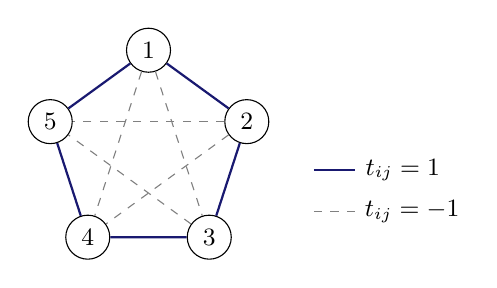
\begin{tikzpicture}[scale=1.05,every node/.style={font=\small}]
  \foreach \i/\angle in {1/90,2/18,3/-54,4/-126,5/162}
    \node[circle,draw,fill=white,inner sep=3pt] (v\i) at (\angle:1.25) {$\i$};
  \foreach \i/\j in {1/3,1/4,2/4,2/5,3/5}
    \draw[dashed,gray] (v\i)--(v\j);
  \foreach \i/\j in {1/2,2/3,3/4,4/5,5/1}
    \draw[thick,MidnightBlue] (v\i)--(v\j);
  \draw[thick,MidnightBlue] (2,-.2)--(2.5,-.2)
    node[right,black] {$t_{ij}=1$};
  \draw[dashed,gray] (2,-.7)--(2.5,-.7)
    node[right,black] {$t_{ij}=-1$};
\end{tikzpicture}
\caption{The five-cycle determining the noninitial off-diagonal entries
of the cubic matrix $T$. Solid edges contribute $\omega$ and dashed edges
contribute $\omega^{-1}$. The diagonal and the initial row and column
consist of ones.}
\label{fig:cubic-cycle}
\end{figure}

The classification also settles the Fourier-vanishing conjecture of
Matolcsi, Ruzsa, and Weiner~\cite[Conjecture~2.3]{MatolcsiRuzsaWeiner2013}.
Here equivalence means multiplication of rows and columns by unit
complex numbers and permutation of rows and columns. The matrix $T$ is
equivalent to the spectral matrix $S_6$ displayed
in~\cite[(93)--(94)]{TadejZyczkowski2006}: with our zero-based indices,
$T_{ij}=(S_6)_{p(i),p(j)}$ for
$(p(0),\ldots,p(5))=(0,1,2,5,4,3)$.

\begin{proof}[Proof of Theorem~\ref{thm:fourier}]
If $g_H(\pi\alpha)$ were nonzero for some coordinate permutation $\pi$,
Corollary~\ref{cor:dichotomy} would imply that $H^{\circ2}$ is
Hadamard. Proposition~\ref{prop:cubic-classification} would then make
$H$ equivalent to $T$, a contradiction.
\end{proof}


\section{Complete families and the cubic obstruction}\label{sec:complete-family}

We turn to Theorem~\ref{thm:main}. The first step is to exclude the
cubic alternative from a complete family. We begin with the character
identities that record mutual unbiasedness and completeness.

\subsection{Character identities of a complete family}

Suppose that
\(B_1,\ldots,B_7\) are mutually unbiased orthonormal bases.
For \(r\ne s\), define their transition matrix by
\[
 H_{rs}(i,k)=\sqrt6\,\langle b_{r,i},b_{s,k}\rangle.
\]
Unbiasedness and orthonormality imply that \(H_{rs}\) is Hadamard and that
\(H_{sr}=H_{rs}^*\). With a reference basis \(r\) fixed, we abbreviate
\(H_{rs}\) and \(g_{H_{rs}}\) to \(H_s\) and \(g_s\).

\begin{lemma}\label{lem:basic}
For each fixed reference basis the following identities hold.
First,
\begin{equation}\label{eq:order-two}
 g_s(d)=0\quad(d\in D),
 \qquad
 \sum_{s\ne r}g_s(a)=0\quad(\ord(a)=2).
\end{equation}
For arbitrary charges \(a,b\) and each coordinate \(i\),
\begin{equation}\label{eq:same-matrix}
 \sum_{j=0}^5 g_s(a+e_i-e_j)g_s(b-e_i+e_j)=g_s(a+b).
\end{equation}
The same identity holds with both shifts reversed. For distinct external
bases \(s,t\ne r\),
\begin{equation}\label{eq:different-matrices}
 \sum_{d\in D}g_s(a+d)g_t(b-d)=0.
\end{equation}
\end{lemma}

The complete-set projector identity used in the proof is the
second-moment identity for a complex projective $2$-design; see
Zauner \cite[Satz~2.19]{Zauner1999} and
Klappenecker--R\"otteler \cite[Theorem~3]{KlappeneckerRotteler2005}.
We give the projection argument in our normalization. The character
identities are part of the Fourier approach
\cite{Matolcsi2012,MatolcsiRuzsaWeiner2013}.

\begin{proof}
The first assertion in \eqref{eq:order-two} is row orthogonality.
For the second, let
\(P_{s,k}=b_{s,k}b_{s,k}^*\), and let \(\mathcal D_s^0\) be the complex
space of traceless matrices diagonal in \(B_s\). If \(s\ne t\), then
\[
 \tr\bigl((P_{s,k}-I/6)(P_{t,l}-I/6)\bigr)=0.
\]
The spaces \(\mathcal D_s^0\) are therefore pairwise orthogonal for the
Hilbert--Schmidt inner product. Each has dimension five, and their
dimensions sum to \(35=6^2-1\), the dimension of the traceless matrix
space. Orthogonal projection consequently gives
\begin{equation}\label{eq:projector-identity}
 \tr(XY)=\sum_{s=1}^7\sum_{k=0}^5
       \tr(XP_{s,k})\tr(YP_{s,k})
 \qquad(\tr X=\tr Y=0).
\end{equation}
This is a complex bilinear identity: it follows by pairing the
complex-linear projection formula for \(X\) with \(Y\).

Any order-two charge is a sum \(d_1+d_2\) of two members of \(D\).
For \(s\ne r\), write \(h_k\) for the \(k\)th column of \(H_s\).
In basis \(B_r\), choose off-diagonal matrix units \(X,Y\) whose traces
against \(P_{s,k}\), for \(s\ne r\), are respectively
\(h_k^{d_1}/6\) and \(h_k^{d_2}/6\). For example,
\(d_1=e_i-e_j\) corresponds to \(X=E_{ji}\).
Since \(d_1+d_2\) has order two, \(d_2\ne-d_1\), so
\(\tr(XY)=0\). The reference basis contributes zero to
\eqref{eq:projector-identity}, and each external basis contributes
\(g_s(d_1+d_2)/6\). This proves the second identity in
\eqref{eq:order-two}.

For \eqref{eq:same-matrix}, expand the two character sums and write
\(x,y\) for their sampled columns. The left-hand side is
\[
 \frac1{36}\sum_{x,y}x^ay^b\frac{x_i}{y_i}
                 \sum_{j=0}^5\frac{y_j}{x_j}.
\]
The inner sum is \(6\) when \(x=y\) and zero otherwise, by column
orthogonality. The result is \(g_s(a+b)\). Conjugating the inner
orthogonality relation proves the version with reversed shifts.

Finally, if \(x\) is a column of \(H_s\) and \(y\) a column of \(H_t\),
their inner-product squared modulus is six. Hence
\[
 \sum_{d\in D}(x/y)^d
 =\left|\sum_{i=0}^5\frac{x_i}{y_i}\right|^2-6=0.
\]
Expanding the products of \(g_s\) and \(g_t\) proves
\eqref{eq:different-matrices}.
\end{proof}

The identities for one matrix hold for every Hadamard matrix.
The order-two sum in \eqref{eq:order-two} uses the completeness of the
seven-basis set. The later mixed identities retain this completeness
information through averaging over the six external bases.

\subsection{The cubic-pair obstruction}

Brierley and Weigert proved the stronger fact that the standard basis
and the basis defined by $T/\sqrt6$ cannot be extended by a third
mutually unbiased basis
\cite[Section~4.1 and Table~1]{BrierleyWeigert2009Constructing}.
The following proposition gives an exact Fourier derivation of the
complete-family exclusion needed here.

\begin{proposition}\label{prop:cubic-exclusion}
In a set of seven mutually unbiased bases in $\C^6$, no transition
Hadamard matrix $H$ can have $H^{\circ2}$ Hadamard.
\end{proposition}

To prove the proposition, suppose that such a pair occurs. By
Proposition~\ref{prop:cubic-classification}, rephasing and reordering
its basis vectors allows us to take its transition matrix to be $T$.
These operations preserve every mutual unbiasedness condition.
Use the first basis of this pair as reference, and call the other
five transition matrices $K_1,\ldots,K_5$. Define
\[
 f(b)=\frac15\sum_{s=1}^5g_{K_s}(b),\qquad G(b)=g_T(b).
\]
Lemma~\ref{lem:basic} gives $f(b)=G(b)=0$ at order one, and
Equation~\eqref{eq:order-two} gives
\begin{equation}\label{eq:cubic-order-two}
 f(b)=-\frac15G(b)\qquad(\ord(b)=2).
\end{equation}
Equation~\eqref{eq:different-matrices}, applied with its second charge
equal to $-c$ and then averaged over $K_1,\ldots,K_5$, gives
\begin{equation}\label{eq:cubic-cross}
 \sum_{d\in D}f(a+d)\overline{G(c+d)}=0
 \qquad\text{for all balanced }a,c.
\end{equation}
Let
\begin{equation}\label{eq:cubic-S}
 S(b)=\frac1{6!}\sum_{\pi\in S_6}
       \Ree\bigl(f(\pi b)\overline{G(\pi b)}\bigr).
\end{equation}
Because $f(-b)=\overline{f(b)}$ and likewise for $G$, this average
also equals the average over the distinct elements of the signed
permutation orbit of $b$.

Every entry of $T$ has cube one, so $G(3d)=1$ for $d\in D$.
The signed permutation orbit of $3(e_5-e_0)$ is precisely
$\{3d:d\in D\}$. If $z$ is a uniformly sampled column of a uniformly
sampled matrix among $K_1,\ldots,K_5$, then $\E z^b=f(b)$. Consequently
\begin{equation}\label{eq:cubic-positivity}
 0\le\E\left|\sum_{i=0}^5z_i^3\right|^2
 =6+\sum_{d\in D}f(3d)
 =6+30S\bigl(3(e_5-e_0)\bigr).
\end{equation}
Thus this orbit average must be at least $-1/5$. We will use
\eqref{eq:cubic-cross} to compute it and contradict this lower bound.
The next lemma concerns $T$ alone; it lets us calculate the coefficients
of those identities one permutation orbit at a time.

\subsection{Symmetries of the cubic matrix}

The row-permutation symmetry below also follows from the semilinear
automorphism group determined by Gillespie, \'O Cath\'ain, and Praeger
\cite[Proposition~2]{GillespieOCathainPraeger2018}. We give a direct
proof using the five-cycle classification.

\begin{lemma}\label{lem:cubic-symmetry}
Every permutation of the rows of $T$ can be completed to a symmetry
of $T$ by column permutations, row and column phase factors, and,
if necessary, complex conjugation. Consequently $|G(b)|$ is constant
on each orbit of balanced charges under permutations and negation.
\end{lemma}

\begin{proof}
A symmetry operation consists of row and column permutations, a choice
of whether to conjugate, and row and column phase factors that send $T$
to itself. Normalize the phase factor of output row zero to one.
The all-one output row and column then determine all the other phase
factors, removing the freedom to multiply the row factors by a common
phase and the column factors by its inverse.

Choose an initial row and column in $36$ ways, choose whether to
conjugate, and dephase at the chosen row and column.
Proposition~\ref{prop:cubic-classification} applies again. After matching
the additional ones on the diagonal, there are exactly $10$ orders of the remaining rows that,
together with the matching column orders, make the plus graph the
specified five-cycle: choose its initial vertex and its direction.
This constructs $36\cdot2\cdot10=720$ symmetry operations. Their row and
column permutations recover the chosen initial row and column as the
source indices sent to position zero; together with the conjugation
choice, their remaining orders recover the chosen cycle isomorphism.
Thus these are distinct normalized operations.

We show that their induced row permutations are distinct. Work with
exponents modulo three, and write $t_j=(t_{ij})_{i=0}^5$ for column $j$
of the exponent matrix. A symmetry fixing the row order acts on the
set $X=\{t_0,\ldots,t_5\}$ as
\[
 X\longmapsto sX+u,\qquad s\in\{1,-1\}.
\]
Indeed, because row zero has only zero exponents, the column phase
factors are common and may be absorbed into the row factors. The
remaining row factors have exponents modulo three, and the image of
the zero column shows that $u\in X$.

For $j\ne0$, column $t_j$ has exactly one zero in its noninitial
positions, at position $j$. Hence $-t_j\notin X$: its zero would force
it to equal $t_j$, which it does not. A nonzero translation preserving
$X$ would contain both $u$ and $2u=-u$, and is therefore impossible.
Negation with $u=0$ is impossible for the same reason.

Finally suppose $s=-1$ and $u=t_x\ne0$. Choose a neighbor $y$ of $x$
on the five-cycle, and let $z$ be their common non-neighbor. Directly
from \eqref{eq:cubic-matrix}, $t_x-t_y$ has its unique noninitial zero
at position $z$: at the other two positions outside $\{x,y,z\}$,
exactly one of $x,y$ is adjacent to that vertex, so the differences
are $\pm2$, hence nonzero modulo three. Were $t_x-t_y$ a column, it
would have to be $t_z$. But at
positions $x,y$ the former has entries $-1,1$, while $t_z$ has entries
$-1,-1$, a contradiction modulo three. Thus the only symmetry fixing
the row order is the identity, after the irrelevant common phase
normalization. Two of the $720$ operations with the same row
permutation would have such a quotient, so their row permutations
are all distinct. They exhaust the $720$ possible row permutations.

For a balanced charge, column phases cancel in the defining
character, while row phases multiply it by a unit complex number.
Conjugation conjugates the character. These observations prove the
last assertion, including negation since $G(-b)=\overline{G(b)}$.
\end{proof}

\subsection{Coefficients of the cross identities}

Let
\[
 a=(-1,-1,0,0,1,1),\qquad c=(0,0,0,0,-1,1),
\]
and let $\mathcal O$ be the set of distinct simultaneous permutations
$(A,C)$ of $(a,c)$.
Apply \eqref{eq:cubic-cross} to every $(A,C)\in\mathcal O$, multiply
by $\overline{G(A-C)}$, sum, and take real parts. To record the
coefficients explicitly, set
\[
 Q(b)=\sum_{\substack{(A,C)\in\mathcal O\\b-A\in D}}
                 G(A-C)G(b-A+C).
\]
The resulting equality is
\[
 \sum_b\Ree\bigl(f(b)\overline{Q(b)}\bigr)=0,
\]
where the sum is finite. For a complex number $z$, write
$z^{[1]}=z$ and $z^{[-1]}=\overline z$. Conjugacy of $f$ permits
symmetrizing the coefficient as
$R(b)=(Q(b)+\overline{Q(-b)})/2$: replacing $b$ by $-b$ in the finite
sum above and averaging leaves it unchanged. Explicitly,
\begin{equation}\label{eq:cubic-R}
 R(b)=\frac12
 \sum_{\substack{(A,C)\in\mathcal O,\ \epsilon\in\{-1,1\}\\
                  \epsilon b-A\in D}}
 \bigl[G(A-C)G(\epsilon b-A+C)\bigr]^{[\epsilon]}.
\end{equation}
We have therefore obtained the weighted cross identity
\begin{equation}\label{eq:cubic-weighted-cross}
 \sum_b\Ree\bigl(f(b)\overline{R(b)}\bigr)=0.
\end{equation}
Its coefficients depend only on $T$. We now calculate them.

The following table lists representatives $w_j$ of every balanced
charge of order at most three, up to permutation and negation. The
integer triples in its last two columns satisfy
\begin{equation}\label{eq:cubic-count-interpretation}
 6G(w_j)=\sum_{m=0}^2N_m\omega^m,
 \qquad
 72R(w_j)=\sum_{m=0}^2U_m\omega^m.
\end{equation}
\begin{table}[htbp]
\centering
\small
\begin{tabular}{@{}rlcc@{}}
\toprule
$j$&$w_j$&$(N_0,N_1,N_2)$&$(U_0,U_1,U_2)$\\
\midrule
0&$(-3,0,0,0,0,3)$&$(6,0,0)$&$(0,0,0)$\\
1&$(-3,0,0,0,1,2)$&$(2,2,2)$&$(0,0,0)$\\
2&$(-3,0,0,1,1,1)$&$(3,0,3)$&$(0,0,0)$\\
3&$(-2,-1,0,0,1,2)$&$(4,1,1)$&$(60,42,42)$\\
4&$(-2,-1,0,1,1,1)$&$(2,2,2)$&$(144,144,144)$\\
5&$(-2,0,0,0,0,2)$&$(2,2,2)$&$(0,0,0)$\\
6&$(-2,0,0,0,1,1)$&$(3,3,0)$&$(180,180,72)$\\
7&$(-1,-1,-1,1,1,1)$&$(3,3,0)$&$(540,540,216)$\\
8&$(-1,-1,0,0,1,1)$&$(4,1,1)$&$(480,336,336)$\\
9&$(-1,0,0,0,0,1)$&$(2,2,2)$&$(576,576,576)$\\
10&$(0,0,0,0,0,0)$&$(6,0,0)$&$(0,0,0)$\\
\bottomrule
\end{tabular}
\caption{Exact cube-root counts for $G$ and $R$.}
\label{tab:cubic-counts}
\end{table}

Here is an explicit summation rule reproducing
Table~\ref{tab:cubic-counts}. Put
\[
 v(b,k)=\sum_{i=0}^5 b_i t_{ik}\pmod3,
\]
with residues in $\{0,1,2\}$. For each input $b=w_j$, initialize two
separate arrays $N,U$ of three zero integers and apply these loops:
\begin{quote}
\begin{verbatim}
for k = 0,...,5:
    N[v(b,k)] += 1
for p,q = 0,...,5 with p != q:
    for 0 <= h < i <= 5 with {h,i} disjoint from {p,q}:
        A = e_p + e_q - e_h - e_i
        u = 2*e_p - e_h - e_i
        for s in {-1,1} with s*b - A in D:
            for k,l = 0,...,5:
                U[(s*(v(u,k) + v(s*b-u,l))) mod 3] += 1
\end{verbatim}
\end{quote}
Indeed, the $30\binom42=180$ pairs in $\mathcal O$ are uniquely
parametrized by
\[
 A=e_p+e_q-e_h-e_i,\qquad C=e_q-e_p,
\]
with precisely the conditions used in the loops; thus $u=A-C$.
Each product of two $G$ terms contributes $36$ cube roots with
coefficient $1/36$, and the factor $1/2$ in
\eqref{eq:cubic-R} accounts for the denominator $72$ in
\eqref{eq:cubic-count-interpretation}.

For example, row $3$ gives
$G(w_3)=(4+\omega+\omega^2)/6=1/2$ and
$R(w_3)=(60+42\omega+42\omega^2)/72=1/4$.
Using $1+\omega+\omega^2=0$ in every row gives
\begin{equation}\label{eq:cubic-R-multipliers}
 R(b)=\lambda_jG(b),\qquad
 \lambda_3=\tfrac12,\quad \lambda_6=3,\quad
 \lambda_7=9,\quad \lambda_8=4,
\end{equation}
on the signed permutation orbit of $w_j$, and $R(b)=0$ on all other
orbits. To justify extending the representative calculation, observe
that every factor in \eqref{eq:cubic-R} has a balanced charge. Its
column phases therefore cancel. The two charges in each product add
to $\epsilon b$, so after the prescribed conjugation its row phase
factor is exactly the factor for $G(b)$. Row permutations preserve
the full set $\mathcal O$, and conjugation conjugates both $R$ and $G$.
Lemma~\ref{lem:cubic-symmetry} therefore gives the asserted covariance
on every orbit; also $R(-b)=\overline{R(b)}$. No other orders can occur
in the support of $R$, since $\epsilon b=A+d$ with
$\ord(A)=2$ and $d\in D$ implies $\ord(b)\le3$.

\subsection{The contradiction}

\begin{proof}[Completion of the proof of Proposition~\ref{prop:cubic-exclusion}]
Write $S_j=S(w_j)$ for the representatives in Table~\ref{tab:cubic-counts}.
The orbit sizes for $j=3,6,7,8$ are respectively
$360,120,20,90$. By \eqref{eq:cubic-R-multipliers}, their coefficients in
\eqref{eq:cubic-weighted-cross}
are $180,360,180,360$. Dividing by $180$ proves
\begin{equation}\label{eq:cubic-first-relation}
 S_3+2S_6+S_7+2S_8=0.
\end{equation}

Table~\ref{tab:cubic-counts} and Lemma~\ref{lem:cubic-symmetry} imply
\[
 S_1=S_4=S_5=S_9=0.
\]
At types $6$ and $8$ the squared modulus of $G$ is $1/4$, so
\eqref{eq:cubic-order-two} gives
\begin{equation}\label{eq:cubic-known-S}
 S_6=S_8=-\frac1{20}.
\end{equation}

Next take $a=c=w_5$ in \eqref{eq:cubic-cross} and average over
coordinate permutations. Do the same with $a=c=w_8$. Classifying the
$30$ charges $w_j+d$, $d\in D$, by their signed permutation orbits
gives the following counts:
\[
\begin{array}{c|rrrrrrrr}
 &0&1&3&4&6&7&8&9\\\hline
 w_5+D&1&8&12&0&8&0&0&1\\
 w_8+D&0&0&4&8&4&2&8&4.
\end{array}
\]
These counts can be obtained simply by adding each of the $30$
vectors $e_i-e_j$ to the displayed representatives and sorting the
coordinates, allowing a simultaneous change of sign. Averaging
over permutations turns each resulting charge into its orbit
average in \eqref{eq:cubic-S}. Substituting the known values gives
\begin{equation}\label{eq:cubic-last-relations}
 S_0+12S_3=\frac25,
 \qquad 4S_3+2S_7=\frac35.
\end{equation}
Together, \eqref{eq:cubic-first-relation},
\eqref{eq:cubic-known-S}, and \eqref{eq:cubic-last-relations} yield
\[
 S_3=S_7=\frac1{10},\qquad S_0=-\frac45.
\]

Since $w_0=3(e_5-e_0)$, equation~\eqref{eq:cubic-positivity} now gives
\[
 \E\left|\sum_{i=0}^5z_i^3\right|^2
 =6+30S_0=-18,
\]
contradicting nonnegativity. This proves the proposition.
\end{proof}

\section{Mixed moments and the remaining case}\label{sec:mixed}

Suppose that a complete set of seven mutually unbiased bases exists and that
its transition matrices satisfy
\begin{equation}\label{eq:all-M}
 g_{H_{rs}}(P\alpha)=0
 \qquad(r\ne s,\;P\text{ a coordinate permutation}).
\end{equation}
We seek a nonnegative averaged quadratic form whose expansion in bounded
moments has a strictly negative upper bound. Corollary~\ref{cor:dichotomy} and
Proposition~\ref{prop:cubic-exclusion} will then exclude a complete set.

\subsection{Sampling and positive forms}

Choose a reference basis index $r$ uniformly from the seven indices. Given
$r$, choose independently a uniform permutation $\sigma$ of its six
coordinates and a uniform bijection $\pi$ from $\{0,\ldots,5\}$ to the
six other basis indices. In this section write
\[
 H_s(i,k)=\sqrt6\,\langle b_{r,\sigma(i)},b_{\pi(s),k}\rangle,
 \qquad g_s=g_{H_s}.
\]
The column order within each basis may remain fixed: each $g_s$ already
averages over all six columns.
For labels $\mathbf s=(s_1,\ldots,s_n)$ and balanced charges
$\mathbf a=(a_1,\ldots,a_n)$ with $\sum_j a_j=0$, define
\begin{equation}\label{eq:mixed-moment}
 \mathcal M(\mathbf s;\mathbf a)
   =\E\,\Ree\!\left(\prod_{j=1}^n g_{s_j}(a_j)\right).
\end{equation}
Equal labels always denote the same matrix. The marginal assignment of any
$l$ distinct labels is a uniform injection into the six nonreference
bases. Thus the definition does not depend on which unused labels are
included in the sampled bijection. The empty product has moment~$1$.

We also use the ordered-pair average of the injective moments of
Section~\ref{sec:pair}:
\begin{equation}\label{eq:average-pair-moment}
 m(A)=\frac1{42}\sum_{r\ne s}m_{H_{rs}}(A),
 \qquad
 H_{rs}(i,k)=\sqrt6\,\langle b_{r,i},b_{s,k}\rangle.
\end{equation}
Here $m_H$ is the real injective moment with the transpose averaging
specified there. All these actual moments obey
\begin{equation}\label{eq:moment-bounds}
 |m(A)|\le1,\qquad |\mathcal M(\mathbf s;\mathbf a)|\le1.
\end{equation}
For the first inequality the integrand has modulus one. For the second,
each $g_s(a)$ is an average of six numbers of modulus one.

The next construction expresses the real parts of Gram entries as linear
combinations of three-factor mixed moments. The third factor comes from
one column shared by all the functions.

In addition to the preceding sampling, choose a uniform column $z$ of
$H_0$. For every balanced charge $a$, define functions on this probability
space by
\begin{equation}\label{eq:F-functions}
 F_0(a)=g_0(a)z^{-a},\qquad
 F_1(a)=\left(\frac15\sum_{s=1}^5g_s(a)\right)z^{-a}.
\end{equation}
The same sampled column $z$ is used in every function $F_t(a)$.
This use of moments and positive Gram forms follows the broader
polynomial-optimization approach to MUBs
\cite{BrierleyWeigert2010SDP,GriblingPolak2024}; the shared-column
functions above specify the particular forms used here.

In the formulas below, an index $1$ on $F$ denotes the average over five
bases in \eqref{eq:F-functions}; a label $1$ in $\mathcal M$ denotes a
representative of those bases after taking expectation.

\begin{lemma}[Gram entries]\label{lem:gram}
For balanced $a,v$, put $\mathbf b=(a,-v,v-a)$. If
$(s,t)\in\{0,1\}^2$ and $(s,t)\ne(1,1)$, then
\begin{equation}\label{eq:gram-first}
 \Ree\,\E\bigl(F_s(a)\overline{F_t(v)}\bigr)
       =\mathcal M((s,t,0);\mathbf b).
\end{equation}
For the remaining case,
\begin{equation}\label{eq:gram-second}
 \Ree\,\E\bigl(F_1(a)\overline{F_1(v)}\bigr)
   =\frac15\mathcal M((1,1,0);\mathbf b)
    +\frac45\mathcal M((1,2,0);\mathbf b).
\end{equation}
\end{lemma}

\begin{proof}
Conditioning first on all the matrices and averaging over $z$ gives
$\E_z z^{v-a}=g_0(v-a)$. In a term with exactly one $F_1$, the five
summands have the same expectation by label exchangeability. In a term
with two $F_1$ factors, expand the two sums independently. Of the $25$
ordered choices of labels from $\{1,\ldots,5\}$, five have equal labels
and twenty have distinct labels. Their marginal distributions give
\eqref{eq:gram-second}. This averaging removes the auxiliary column
completely. A zero charge contributes $g_s(0)=1$ and may be deleted;
removing any unused label preserves the uniform injection law already
described.
\end{proof}

\subsection{Reducing the Gram entries}

The three-factor moments in Lemma~\ref{lem:gram} can be simplified using
symmetry, character vanishing, and the identities of a complete family.
When all factors refer to one matrix, the injective moments and equations
from Section~\ref{sec:pair} apply as well.

\Needspace{7\baselineskip}
\begin{lemma}[Mixed-moment reductions]\label{lem:mixed-reductions}
Under \eqref{eq:all-M}, the following operations and identities are valid.
\begin{enumerate}[label=\textup{(\roman*)}]
 \item A common coordinate permutation of all charges, simultaneous
 negation of all charges, a simultaneous reordering of factors and their
 labels, and an arbitrary injective renaming of the used labels preserve
 \eqref{eq:mixed-moment}. A zero charge factor may be omitted. Coordinates
 on which every charge is zero may also be omitted, with the remaining
 coordinates interpreted as a uniform injection into the six row positions.

 \item The moment vanishes if any charge has order one or is a coordinate
 permutation of $\alpha$.

 \item Suppose that $a_j$ has order two and its label $s_j$ occurs only
 once. Let $S$ be the set of distinct used labels and $l=|S|$. For each
 $t\in S\setminus\{s_j\}$, let $\mathbf s^{j\to t}$ be obtained from
 $\mathbf s$ by replacing $s_j$ with $t$. Then
 \begin{equation}\label{eq:singleton-reduction}
 \mathcal M(\mathbf s;\mathbf a)
 =-\frac1{7-l}\sum_{t\in S\setminus\{s_j\}}
       \mathcal M(\mathbf s^{j\to t};\mathbf a).
 \end{equation}

 \item If all labels are equal, the moment is a linear combination of
 the pair moments \eqref{eq:average-pair-moment}. More precisely, let
 $A$ have columns $a_1,\ldots,a_n$, after removing its zero rows. For a
 set partition $\mathcal P$ of $\{1,\ldots,n\}$, let $A_{\mathcal P}$
 have one column $\sum_{j\in B}a_j$ for each block $B\in\mathcal P$.
 Then
 \begin{equation}\label{eq:single-label-partitions}
 \mathcal M((s,\ldots,s);\mathbf a)
 =\sum_{\substack{\mathcal P\text{ a set partition}\\|\mathcal P|\le6}}
       \frac{(6)_{|\mathcal P|}}{6^n}\,m(A_{\mathcal P}),
 \end{equation}
 where $(6)_k=6\cdot5\cdots(6-k+1)$. Zero rows or columns in
 $A_{\mathcal P}$ may be deleted as in Section~\ref{sec:pair}.

 \item For balanced $a,b,c$ with $a+b+c=0$,
 \begin{align}
 &\sum_{j=0}^5
 \mathcal M\bigl((s,s,u);
       (a+e_i-e_j,b-e_i+e_j,c)\bigr)
   =\mathcal M\bigl((s,u);(a+b,c)\bigr),
       \label{eq:mixed-same}\\
 &\sum_{d\in D}
 \mathcal M\bigl((s,t,u);(a+d,b-d,c)\bigr)=0
       \qquad(s\ne t).
       \label{eq:mixed-different}
 \end{align}
 Equation~\eqref{eq:mixed-same} also holds with the signs of both shifts
 reversed. The third label $u$ may coincide with another label.
\end{enumerate}
\end{lemma}

\begin{proof}
Uniform sampling gives the coordinate and label symmetries in (i), while
commutativity gives factor reordering. Simultaneous negation conjugates
the whole product, leaving its real part unchanged. A zero charge gives
$g_s(0)=1$. Removing unused labels or coordinates leaves a uniform
injection on those retained. Part (ii) follows from Hadamard
orthogonality and \eqref{eq:all-M}. In particular, a permuted $\alpha$
has six nonzero coordinates; deleting zero coordinate rows cannot change
whether a charge is of this type.

For (iii), fix $r$, the row permutation, and the bases assigned to the
$l-1$ other used labels. There are $6-(l-1)=7-l$ available bases for the
singleton label. For this fixed row order, let $\widetilde g_v$ denote
the character average for the external basis $v$. Equation~\eqref{eq:order-two} gives
\[
 \sum_{\substack{v\ne r\\v\text{ not already assigned}}}
       \widetilde g_v(a_j)
 =-\sum_{t\in S\setminus\{s_j\}}g_t(a_j),
\]
with the same row order throughout. Multiply by the other factors and
average over the remaining choices. The marginal distribution of the
$l-1$ retained labels is exactly the distribution defining each moment
on the right of \eqref{eq:singleton-reduction}.

For (iv), expand each $g_s$ as its column average and group the resulting
$n$ column choices by their equality partition. A partition with $k$
blocks has $(6)_k$ distinct assignments to its blocks, out of $6^n$
choices, giving the displayed coefficient. The retained rows are sampled
injectively. It remains to justify the transpose averaging in $m(A)$.
The marginal ordered pair of bases is uniform, and
$H_{sr}=\overline{H_{rs}}^{\,\mathsf T}$. Exchanging $r$ and $s$
exchanges the row and column injections and sends an exponent matrix
$A$ to $-A^{\mathsf T}$. Negating all exponents conjugates the monomial,
leaving its real part unchanged. Thus the ordered-pair average is already
invariant under transposition. This proves \eqref{eq:single-label-partitions}, including
the transpose convention in \eqref{eq:average-pair-moment}.

Finally, multiply \eqref{eq:same-matrix} or
\eqref{eq:different-matrices} by $g_u(c)$ and take real expectations.
These pointwise identities give (v).
\end{proof}

In the finite calculation below, a mixed key consists of its factor
labels and the matrix whose columns are its charges. The reductions in
Lemma~\ref{lem:mixed-reductions} apply to these keys. Single-label keys
are expanded into the moments $m(A)$, and the pair relations from
Section~\ref{sec:pair} may then be used. If a single-label expression
vanishes by part (ii), its expansion also gives a valid homogeneous
relation among the $m(A)$. These steps preserve the interpretation of
every remaining symbol as an actual moment.

\subsection{The six positive forms}

Here are the finite collections of functions and integer weights used
in the certificate. The exact data are the literal list named
\texttt{data} in Appendix~\ref{app:code}, also supplied in the companion
file \texttt{certificate/verify.py}. Each record has the form
\[
 (\lambda,\ \texttt{ws},\ e_\lambda,\ \texttt{a}).
\]
The list $\texttt{ws}=((t_0,v_0),\ldots,(t_{m-1},v_{m-1}))$ specifies
$m$ pairs with $t_i\in\{0,1\}$ and balanced $v_i\in\Z^6$.
The integer list $\texttt{a}$ specifies a symmetric $m\times m$ matrix
$Z_\lambda$ by its lower triangle in row order: with zero-based list
indices,
\begin{equation}\label{eq:Z-encoding}
 (Z_\lambda)_{ij}=(Z_\lambda)_{ji}
       =\texttt{a}_{\,i(i+1)/2+j}
       \qquad(0\le j\le i<m).
\end{equation}
Thus the data define the matrices and lists without any optimization or
choice of numerical tolerances. Their sizes and scales are
\begin{center}
\begin{tabular}{@{}lrr@{}}
\toprule
$\lambda$ & $m$ & $e_\lambda$\\
\midrule
$(1,1,1,2)$ & 5  & 14\\
$(1,1,3)$   & 21 & 13\\
$(1,2,2)$   & 11 & 13\\
$(1,4)$     & 27 & 14\\
$(2,3)$     & 22 & 14\\
$(5)$       & 12 & 15\\
\bottomrule
\end{tabular}
\end{center}

For each of these six lists of row lengths $\lambda$, place the positions
$1,\ldots,5$, in order, in successive left-justified rows of lengths
$\lambda_1,\lambda_2,\ldots$. Let $R_\lambda$ consist of permutations
within these rows, and let $C_\lambda$ consist of permutations within
the resulting columns. Both groups act on $\{0,\ldots,5\}$ by fixing
position~$0$. Our convention for their action on charges is
\[
 (P_pv)_i=v_{p(i)}.
\]
These signed row and column permutation sums are the usual
Young-symmetrizer construction. Symmetry reduction of positive Gram
forms is developed generally in \cite{GatermannParrilo2004} and for MUB
moment problems in \cite{GriblingPolak2024}. Here the finite sums are
given explicitly, so their use requires no representation-theoretic
decomposition theorem.
Define the vector $Y_\lambda$ by
\begin{equation}\label{eq:Young-functions}
 (Y_\lambda)_i
    =\sum_{\substack{p\in R_\lambda\\q\in C_\lambda}}
          \operatorname{sgn}(q)\,
          F_{t_i}(P_pP_qv_i)
       \qquad(0\le i<m).
\end{equation}
In particular, $(P_pP_qv)_i=v_{q(p(i))}$, which is the order implemented
by \texttt{perm(perm(v,q),p)} in the appendix. Formula
\eqref{eq:Young-functions} defines a finite linear combination of the
functions \eqref{eq:F-functions} for every listed pair.

\begin{proposition}[Mixed-moment certificate]\label{prop:mixed-certificate}
Each matrix $Z_\lambda$ specified above is positive definite. Under the
mixed-moment identities of Lemma~\ref{lem:mixed-reductions}, the forms
\eqref{eq:Young-functions} satisfy
\begin{align}
 5\sum_\lambda 10^{15-e_\lambda}
       \E\bigl(Y_\lambda^*Z_\lambda Y_\lambda\bigr)
 &\le
       \frac{-613302797399911+179721388988719}{6480}
       \label{eq:mixed-certificate}\\
 &=-\frac{2007321335237}{30}<0.\notag
\end{align}
\end{proposition}

\begin{proof}
The exact finite calculations establishing the matrix and coefficient
claims are detailed in Section~\ref{sec:verification}, with their full
integer and rational arithmetic in Appendix~\ref{app:code}. We specify
here the mathematical expansion to which those checks apply.

First expand each $Y_\lambda$ by \eqref{eq:Young-functions}, and replace
every real Gram entry using Lemma~\ref{lem:gram}. Multiplication by
five makes its weights either $5$ or the pair $(1,4)$. Because
$Z_\lambda$ is real symmetric, summing its diagonal contributions and
twice its lower off-diagonal contributions gives the real quantity
$\E(Y_\lambda^*Z_\lambda Y_\lambda)$. The factor
$10^{15-e_\lambda}$ is retained for each block.

Apply the mixed reductions and the homogeneous relations
\eqref{eq:mixed-same}--\eqref{eq:mixed-different}, using the finite
selection of relations with total charge order at most $11$ described
in Section~\ref{sec:verification}. That selection only restricts which
valid relations are used. The exact substitutions give
\begin{equation}\label{eq:mixed-residual}
 5\sum_\lambda 10^{15-e_\lambda}
       \E\bigl(Y_\lambda^*Z_\lambda Y_\lambda\bigr)
    = f+\sum_{\rho\in\mathcal R}\beta_\rho X_\rho,
\end{equation}
where each $X_\rho$ is a nonconstant symbol representing one of the
original moments $m(A)$ or $\mathcal M(\mathbf s;\mathbf a)$, and
\begin{equation}\label{eq:mixed-coefficients}
 f=-\frac{613302797399911}{6480},\qquad
 \sum_{\rho\in\mathcal R}|\beta_\rho|
     =\frac{179721388988719}{6480}.
\end{equation}
The linear-algebra verification in Section~\ref{sec:verification}
proves that these substitutions follow from the chosen equations.
The bounds \eqref{eq:moment-bounds} applied to
\eqref{eq:mixed-residual} now prove
\eqref{eq:mixed-certificate}.

For each $Z_\lambda$, the exact Schur-complement calculation in
Section~\ref{sec:verification} verifies positive pivots and hence positive
definiteness.
\end{proof}

\begin{proof}[Completion of the proof of Theorem~\ref{thm:main}]
If seven mutually unbiased bases existed, Corollary~\ref{cor:dichotomy}
would give case (M) or case (C) for each transition matrix.
Proposition~\ref{prop:cubic-exclusion} excludes case (C), so all pairs
satisfy \eqref{eq:all-M} and the preceding construction applies.
For a complex vector $Y=x+\mathrm i y$ and a real symmetric positive
definite matrix $Z$,
\[
 Y^*ZY=x^{\mathsf T}Zx+y^{\mathsf T}Zy\ge0.
\]
Consequently the left side of \eqref{eq:mixed-certificate} is
nonnegative. Its strictly negative upper bound is a contradiction.
This proves Theorem~\ref{thm:main}.
\end{proof}

\section{Exact verification of the two certificates}
\label{sec:verification}

We now give the finite calculations establishing
Propositions~\ref{prop:pair-certificate} and~\ref{prop:mixed-certificate}.
The complete program and all its data are printed in
Appendix~\ref{app:code}.  It specifies the integer
matrices, coordinate orders, and finite enumerations used below.  All
arithmetic that certifies an equality or inequality is integer or rational
arithmetic.  Modular arithmetic supplies candidate substitutions, whose
validity is then checked exactly.
Rational Gram certificates and exact positivity checks are established
methods; see Peyrl--Parrilo \cite[Section~3]{PeyrlParrilo2008}.
Our input matrices are specified integers, and the proof below certifies
the displayed identities directly from those data.

The calculation has three steps.  First, expand each expression in named
moments using the identities already proved.  Next, use a finite set of
true linear equations to substitute for some of these moments.  Finally,
check either that every coefficient vanishes, for the pair certificate, or
that the constant coefficient plus the absolute sum of the remaining
coefficients is negative, for the mixed certificate.  We first justify the
substitutions for arbitrary real moment values, then specify the equations and coefficient checks for each certificate.

\subsection{Exact certification of linear substitutions}

Both certificates use finite systems of linear equations in their moment
coordinates. The same substitution procedure applies to either system.
Include the constant moment as a coordinate, so that every moment equation is
homogeneous in the enlarged coordinate vector.  Clearing denominators
turns the equations into integer rows.  The lists called \texttt{I} in
the program specify a fixed priority order on the coordinates.  This
choice affects the form of the answer and, in the mixed calculation,
the size of its residual coefficient sum; it does not add any relation.

\begin{lemma}[Exact substitutions]
\label{lem:exact-elimination}
Let $W\in\Z^{r\times N}$ consist of selected moment equations after
their denominators have been cleared.  Suppose a set $J$ of $r$ columns gives a square
submatrix $W_J$ invertible modulo a prime.  Put
$F=\{1,\ldots,N\}\setminus J$.  If a rational matrix
$P\in\Q^{N\times N}$ satisfies
\[
 P_{F,F}=I,\qquad P_{*,J}=0,\qquad WP=0,
\]
then every real vector $\mathbf m$ satisfying $W\mathbf m=0$ obeys
$\mathbf m=P\mathbf m$.  Thus the rows of $P$ give valid substitutions
for all coordinates in terms of the coordinates indexed by $F$.
\end{lemma}

\begin{proof}
Invertibility modulo the prime implies that the integer
$\det W_J$ is nonzero.  In the coordinate order $J,F$, write
\[
 W=\begin{pmatrix}W_J&W_F\end{pmatrix},\qquad
 P=\begin{pmatrix}0&P_{J,F}\\0&I\end{pmatrix}.
\]
The exact equality $WP=0$ gives
$P_{J,F}=-W_J^{-1}W_F$.  Every solution of $W\mathbf m=0$ consequently
satisfies $\mathbf m_J=P_{J,F}\mathbf m_F$, while the free coordinates
of $P\mathbf m$ are already $\mathbf m_F$.  This proves the claim over
$\mathbb R$, regardless of whether the moment values are rational.
Equivalently, $P$ has rank $N-r$, its image equals $\ker W$, and its
identity rules make it the identity on that kernel.
\end{proof}

Here is how \texttt{eliminate} verifies the hypotheses of the lemma.
Its first modular elimination uses the prime $1000000007$.  The routine
\texttt{echelon} retains an original integer equation whenever that
equation supplies a new pivot.  These retained equations form $W$.
Each pivot is at the largest remaining coordinate of its row; normalized
elimination therefore proves that $W_J$ is invertible modulo the prime.
Back substitution processes pivot coordinates in ascending order.
When a smaller pivot is removed, its already reduced row contains only
that pivot and free coordinates.  The final rule for a pivot thus has
no other pivot on its right side.

The program then works modulo the further moduli listed in the source,
retaining matching pivot sets, combines coefficients by the Chinese
remainder algorithm, and uses \texttt{rat} to propose rational rules.
These steps preserve the absence of other pivot coordinates.  All
nonpivot coordinates receive explicit identity rules.  Finally, for
each retained integer equation the program substitutes every proposed
rule, clears all denominators, and checks that every integer
coefficient is zero.  This is the exact check $WP=0$ in
Lemma~\ref{lem:exact-elimination}.

Every actual moment vector satisfies the selected equations, so this
check suffices even if additional generated equations have not been
used.  In particular, the modular pivot count is not asserted to be the
full rational rank of the original system.  A prime that conceals an
additional independent equation merely leaves that true equation
unused.  The rational reconstruction and its size threshold are ways
to find a candidate $P$; the exact check and the lemma establish its
validity.

\subsection{Pair equations and the vanishing identity}

For an integer array $A$ with zero row and column sums, put
\[
 \operatorname{wt}(A)=\sum_i\ord(A_{i,*}).
\]
This also equals the sum of the column orders.  Arrays name the real
injective moments $m_H(A)$ of Section~\ref{sec:pair}; the empty array names
the constant moment $1$.  A formal linear expression in these moments is
stored as a finite list of rational coefficients indexed by arrays.
Coefficients at the same index are added, and zero coefficients are
discarded.  These are the operations \texttt{add} and \texttt{lin} in the
program.

The routine \texttt{canonpair} selects a representative using precisely
the symmetries of $m_H$: permutation of either axis, removal of zero
rows and columns, global negation, and transposition.  More explicitly,
after removing zero axes it considers $A,-A,A^{\mathsf T},-A^{\mathsf T}$,
retains orientations with at least as many rows as columns, orders
columns by their positive-part orders, and minimizes over the remaining
column permutations after lexicographically sorting the rows.  Each
operation preserves the moment by its definition and
Lemma~\ref{lem:contraction}.  The degree orders and lexicographic choices
serve only to select consistent names.

Define $U_0(A)$ recursively as a linear expression in representatives
whose nonzero row and column orders are all at least two.  If a row of
$A$, or of $A^{\mathsf T}$, has order one, apply
Lemma~\ref{lem:contraction} in that orientation:
\begin{equation}
 U_0(A)=-\frac{1}{7-p}\sum_{\ell\ne i}U_0(A_{i\to\ell}),
 \qquad p\le6.
 \label{eq:recursive-pair-reduction}
\end{equation}
Canonicalize each contracted array before continuing.  If no such row
exists on either axis, retain its moment as a single coordinate.  The
empty array is retained in the same way.  Every contraction reduces the
sum of the two axis lengths, so this recursion terminates.  This is
\texttt{evpair}; \texttt{expand\_degree1} supplies the unsigned sum of
contractions.  The program checks that every evaluated array has both
dimensions at most six and has zero sums on both axes.

The pair table is formed from formal seven-row equations.  The exact
enumeration restrictions are as follows:
\begin{enumerate}[label=(\roman*)]
 \item Choose a total weight $k\in\{7,8,9,10,11\}$ and a column count
 $q$ with $2\le q\le\min(4,\lfloor k/2\rfloor)$.
 \item Choose nondecreasing sequences of seven row orders
 $(r_0,\ldots,r_6)$ and $q$ column orders $(c_0,\ldots,c_{q-1})$.
 Both sequences sum to $k$, and
 \[
 1\le r_i\le\lfloor k/2\rfloor,
 \qquad 2\le c_j\le\lfloor k/2\rfloor.
 \]
 \item Enumerate integer $7\times q$ arrays with zero row and column
 sums and exactly these orders.  Rows of equal order may be put in
 lexicographic order, and arrays with the same canonical representative
 may be skipped.
\end{enumerate}
The routines \texttt{parts}, \texttt{comps}, and \texttt{allAB} implement
this enumeration.  A row is generated as the difference of disjointly
supported nonnegative compositions of its prescribed order, within the
remaining positive and negative column capacities.  The capacities
enforce the prescribed column orders.  The first row has order one:
seven positive integer row orders with sum at most eleven cannot all
be at least two, and the orders are sorted.

For each retained array, the seven-row boundary case of
Lemma~\ref{lem:contraction} gives the equation
\begin{equation}
 \sum_{\ell=1}^{6}U_0(A_{0\to\ell})=0.
 \label{eq:pair-table-equations}
\end{equation}
Here $0,\ldots,6$ index the formal rows, not coordinates of a charge.
Only the contracted arrays, which have at most six rows, are evaluated.
The checks in \texttt{pairtable} verify the balance, number of formal
rows, and order of the first row before forming this equation.
Skipping an array can only omit an available true equation; the proof
does not require a complete set of moment relations.

Apply Lemma~\ref{lem:exact-elimination} to these equations.  Write
$U(A)$ for the resulting expansion of $U_0(A)$ in the retained moment
coordinates.  For a product used here, with charge columns
$a_1,\ldots,a_n$ and $n\le4$, let
$A_{\mathcal S}$ be the array obtained by adding the columns in each
block of a set partition $\mathcal S$ of $\{1,\ldots,n\}$.  The final
pair expansion is
\begin{equation}
 \sum_{\substack{\mathcal S\text{ a set partition}\\|\mathcal S|\le6}}
 \frac{(6)_{|\mathcal S|}}{6^n}\,U(A_{\mathcal S}).
 \label{eq:verified-partition-expansion}
\end{equation}
This is exactly Lemma~\ref{lem:partitions}.  The routine
\texttt{partition} enumerates set partitions by numbering blocks in
order of first occurrence, and \texttt{rep\_pair} implements
\eqref{eq:verified-partition-expansion}.  The routine \texttt{apair}
first forms the array of charge columns.  It may remove a zero charge
before the expansion, since that removes the factor $g_H(0)=1$.
Deletion of zero coordinate rows is also legitimate: a uniform
injection on the retained positions has the required uniform marginal.

For the pair certificate, \texttt{check\_pair} forms the displayed
polynomial $L_H$ of Proposition~\ref{prop:pair-certificate}, with
coefficients $-1,2,1,1,1$.  It multiplies each monomial by the conjugate
of every monomial, expanding $3|L_H|^2$ through
\eqref{eq:verified-partition-expansion}.  For each of the two stated
charges $q$, it adds the expansion with charge columns
$(\alpha,q,-\alpha,-q)$.  After the exact pair substitutions, the
result has no nonzero coefficient, for either $q$.  This proves the
identity in Proposition~\ref{prop:pair-certificate}; all expressions
used in the check have been identified with their actual averaged
moment values above.

\subsection{Mixed keys and the finite mixed table}

We use the notation $\mathcal M(\mathbf s;\mathbf a)$ and $m(A)$ from
Section~\ref{sec:mixed}.  The latter is the average of $m_H(A)$ over
the ordered basis pairs.  A mixed key consists of a label tuple
$\mathbf s$ and an array $A$ whose columns are the charges.  The array
has at most six nonzero coordinate rows.  Its rows and columns sum to
zero.  The routine \texttt{cmix} chooses representatives by simultaneous
factor and label permutations, renaming labels by order of first
occurrence, sorting the common coordinate rows, global negation, and
removing zero factors and zero coordinate rows.  These are exactly the
symmetries justified in Lemma~\ref{lem:mixed-reductions}.  The separate
tag $(\varnothing,A)$ names the pair moment $m(A)$; the completely empty
key names $1$.

The routine \texttt{evmix} supplies the following recursive expansion
of a key into named moment coordinates:
\begin{enumerate}[label=(\roman*)]
 \item If a charge has order one or is a permutation of $\alpha$, the
 mixed moment is zero.
 \item When at most one label remains, expand the product by
 \eqref{eq:verified-partition-expansion}, now using the averaged pair
 moments $m(A)$, and attach the pair tag to its coordinates.
 If this single-label expression was zero by the preceding rule,
 also record its pair expansion as a zero equation.  These recorded
 equations are stored in \texttt{rows0}.
 \item Otherwise, if an order-two charge has a label occurring exactly
 once among the factors, let $l$ be the number of labels in use and
 replace that label in turn by each of the other $l-1$ labels.  The
 original moment is $-1/(7-l)$ times the sum of the resulting moments.
 Apply the same rules recursively to each term.
 \item If none of these rules applies, retain the key as an original
 mixed-moment coordinate.
\end{enumerate}
The zero rules and the singleton coefficient follow from
Lemma~\ref{lem:mixed-reductions}.  Each singleton replacement decreases
the number of distinct labels.  The single-label use of the pair table
is legitimate because the real average over ordered pairs includes
the required transpose symmetry, as proved in that lemma.

The finite enumeration of triples is given by \texttt{triples(11)}.
For precision, it generates balanced charges $a,b,c\in\Z^6$ with
\[
 \begin{gathered}
 a+b+c=0,\qquad 0\le\ord(c)\le\ord(b)\le\ord(a)\le5,\\
 \ord(a)+\ord(b)+\ord(c)\le11.
 \end{gathered}
\]
Choose $a$ up to a coordinate permutation and sign by taking the lesser
of its sorted entries and the sorted entries of $-a$.  Enumerate all
balanced $b$ of orders at most $\ord(a)$, put $c=-a-b$, and retain those
meeting the displayed restrictions.  Sorting the six rows of the
array $(a,b,c)$ removes common-coordinate duplicates.  Balanced
vectors of a given order are generated by subtracting two
disjointly supported nonnegative compositions of that order, which is
the routine \texttt{vecs}.

For each generated array, \texttt{mixeq} first evaluates all five
equality patterns on its three labels, registering any single-label
zero equations.  It then considers the distinct permutations of the
three charge columns, choosing $a\le b$ lexicographically to avoid
duplicated first-two-column orderings.  Write
\[
 a_{ij}=a+e_i-e_j,\qquad b_{ij}=b-e_i+e_j
 \quad (0\le i,j\le5).
\]
\Needspace{6\baselineskip}
The following equations are included after applying \texttt{evmix} to
every term:
\begin{itemize}
 \item For different first two labels, sum the moments with charges
 $(a_{ij},b_{ij},c)$ over all $i\ne j$, obtaining zero by
 \eqref{eq:different-matrices}.  For nonzero $c$, use the label tuples
 $(0,1,2)$, $(0,1,0)$, and $(0,1,1)$; for $c=0$, use $(0,1,0)$.
 Include this equation only if all $36$ shifted triples have total
 order at most eleven.
 \item For equal first two labels, fix $i$, sum over all six $j$, and
 subtract the moment with charges $(-c,c)$ and labels $(0,u)$, by
 \eqref{eq:same-matrix}.  Use $(0,0,u)$ with $u=0,1$ when $c\ne0$,
 and $u=0$ when $c=0$.  Also use the reversed shifts
 $(a+e_j-e_i,b-e_j+e_i,c)$.  Include each equation only if all its six
 shifted triples have total order at most eleven.
\end{itemize}
The third charge is unchanged in these sums because the equations have
been multiplied by its factor.  On the right side of the equal-label
equation, $a+b=-c$, which explains both remaining charges and the
labels selected by \texttt{s[-2:]} in the source.

Finally add the pair equations recorded in \texttt{rows0}.  All
coordinates encountered by these reductions are registered, including
coordinates that cancel in a particular equation.  With the specified
coordinate order, \texttt{mixtable} applies
Lemma~\ref{lem:exact-elimination} to the nonzero equations.  A vanishing
expression encountered later may still be replaced by zero: its
vanishing is an independently proved rule, whether or not its pair
expansion was used to strengthen this table.  No completeness of the
enumeration, and no vanishing of unlisted higher-order moments, is
assumed.

The exact table dimensions are as follows.  The witness column counts
the independent equations used in Lemma~\ref{lem:exact-elimination}.
\begin{center}
\begin{tabular}{lrrr}
\toprule
Table & Nonzero equations & Coordinates & Witness rows \\
\midrule
Pair  & $8871$  & $909$  & $897$ \\
Mixed & $46041$ & $3429$ & $2767$ \\
\bottomrule
\end{tabular}
\end{center}

\subsection{Positive matrices and the negative bound}

For the mixed certificate, the literal data in Appendix~\ref{app:code}
specify the six lists and lower triangles of the symmetric integer
matrices $Z_\lambda$.  The routine \texttt{makeZ} checks the number of
entries and reconstructs each symmetric matrix.  Positive definiteness
is verified without eigenvalue approximation.  At each step,
\texttt{posdef} writes the remaining matrix as
\[
 B=\begin{pmatrix}C&u\\u^{\mathsf T}&p\end{pmatrix},
 \qquad p>40000,
\]
and replaces it by the exact Schur complement $C-uu^{\mathsf T}/p$.
The identity
\[
 \begin{pmatrix}x\\t\end{pmatrix}^{\!*}
 B\begin{pmatrix}x\\t\end{pmatrix}
 =x^*(C-uu^{\mathsf T}/p)x
   +p\left|t+\frac{u^{\mathsf T}x}{p}\right|^2
\]
shows inductively that positive pivots prove positive definiteness,
also for complex vectors.  All $98$ pivots in the six matrices satisfy
the asserted rational inequality.

The routines \texttt{permsign} and \texttt{polynomial} implement the
signed permutation sums defining $Y_\lambda$ in
Section~\ref{sec:mixed}.  The convention
$(P_pv)_i=v_{p(i)}$ gives
$(P_pP_qv)_i=v_{q(p(i))}$, exactly
\texttt{perm(perm(v,q),p)}.  The routine \texttt{tagmom} uses the Gram
charges $(a,-v,v-a)$ of Lemma~\ref{lem:gram}.  After multiplying the
entire form by five, \texttt{product} assigns weight five unless both
function types are one; in that case the weights for equal and
different external labels are one and four.  The lower-triangle
summation in \texttt{gaps} doubles the off-diagonal terms.  Since the
polynomial coefficients and $Z_\lambda$ are real, its real-moment
expansion equals the full quadratic form for complex $Y_\lambda$.

Consequently the expression formed by \texttt{gaps} is exactly
\[
 \mathcal Q=
 5\sum_\lambda 10^{15-e_\lambda}
       \E\bigl(Y_\lambda^*Z_\lambda Y_\lambda\bigr).
\]
Apply \texttt{evmix} and then the certified mixed substitutions.  On
combining coefficients, we obtain the residual expansion in
\eqref{eq:mixed-residual}, now indexed by the program's moment keys:
\begin{equation}
 \begin{gathered}
 \mathcal Q=c_0+\sum_{K\ne\varnothing}c_K\,\mu_K,\\
 c_0=-\frac{613302797399911}{6480},\qquad
 \sum_{K\ne\varnothing}|c_K|
     =\frac{179721388988719}{6480}.
 \end{gathered}
 \label{eq:exact-residual-coefficients}
\end{equation}
Here $\mu_K$ denotes the original moment named by a retained coordinate;
the notation $K\ne\varnothing$ excludes the completely empty constant
key.  Both equalities of rational coefficients in
\eqref{eq:exact-residual-coefficients} are checked exactly by the
program, as is their strictly negative sum.

It remains to justify the bound on these residual coordinates.  A
tagged pair coordinate is a real average of unit-modulus monomials, so
$|m(A)|\le1$.  A mixed coordinate is a real average of products of
$g_s(a)$, each of absolute value at most one, so
$|\mathcal M(\mathbf s;\mathbf a)|\le1$.  Every coordinate retained by
the substitutions is one of these original moments.  The new linear
combinations occur as expressions in the coordinates, not as newly
named coordinates to which a bound is assigned.  The constant
coordinate is exactly one.  Hence
\[
 0\le\mathcal Q
 \le c_0+\sum_{K\ne\varnothing}|c_K|
 =-\frac{2007321335237}{30}<0.
\]
This proves Proposition~\ref{prop:mixed-certificate}.  Together with
the pair coefficient check, it completes the exact verification of
both certificates using only the finite equations and integer data
specified in Appendix~\ref{app:code}.


\clearpage
\appendix
\section{Complete exact verifier}\label{app:code}

This appendix gives the exact verifier for
Propositions~\ref{prop:pair-certificate} and~\ref{prop:mixed-certificate}.
The cubic character counts are specified by the finite sums and loops
following Table~\ref{tab:cubic-counts}.

The program below uses only the Python standard library and runs with
Python 3.8 or later, with assertions enabled. Its standalone file is
\texttt{verification/verify.py}. The accompanying wrapper
\texttt{verification/run.py} checks that assertions are enabled and that
the verifier has the expected checksum before running it. From the
paper directory, execute
\begin{center}
\texttt{python3 verification/run.py}
\end{center}
The complete expected output is
\begin{lstlisting}[basicstyle=\small\ttfamily,columns=fullflexible,keepspaces=true]
rank table: 8871 909 897
rank table: 46041 3429 2767
-613302797399911/6480 179721388988719/6480 5000000000000000
\end{lstlisting}
In each \texttt{rank table} line, the three entries give the number of
nonzero equations, the number of moment coordinates, and the number of
independent witness rows used for substitution, respectively.
The final line gives the constant coefficient, the sum of
the absolute values of all nonconstant coefficients, and the overall
normalizing scale $5\cdot10^{15}$. Dividing the first two entries by
this scale gives the constant and residual coefficient norm for
$\sum_\lambda 10^{-e_\lambda}\E(Y_\lambda^*Z_\lambda Y_\lambda)$.
Every assertion in the program is checked in integer or rational arithmetic.

\Needspace{4\baselineskip}
For reference, the SHA-256 checksum of \texttt{verification/verify.py} is
\begin{center}\footnotesize\ttfamily
104a7306205b8544c8f913f6afdb59603f2e\allowbreak
04a207c9ac592c383b80eb0e2aa9
\end{center}
The literal \texttt{data} near the end specifies each shape, its ordered
list of function types and charges, its decimal scale exponent, and the
lower triangle of its symmetric integer matrix, in row order.

Equation numbers in the code comments use the original numbering:
the reference in \texttt{expand\_degree1} is to the contractions of
Lemma~\ref{lem:contraction}, and those in \texttt{mixeq} are to
\eqref{eq:same-matrix} and \eqref{eq:different-matrices}.

\lstinputlisting[style=certificate,caption={Complete exact verifier},label={lst:verifier}]{certificate/verify.py}

\clearpage
\bibliographystyle{plain}
\bibliography{references/references}
\end{document}
